% !TeX root = ..\rapport_13_2.tex
\section{Design by contract}

\subsection{generateProjectNumber}
pre: 
\begin{equation}
    pr \neq null \land date \neq null
\end{equation}
post:
\begin{equation}
    \text{result }=\{s|\exists p \in projectRepository.getProjectNumbers : s \in p \land p = largestProjectNumber(date)\}
\end{equation}
Med asserts ser det ud som følger:
\begin{figure}[H]
    \centering
    \caption{generateProjectNumber med asserts}
    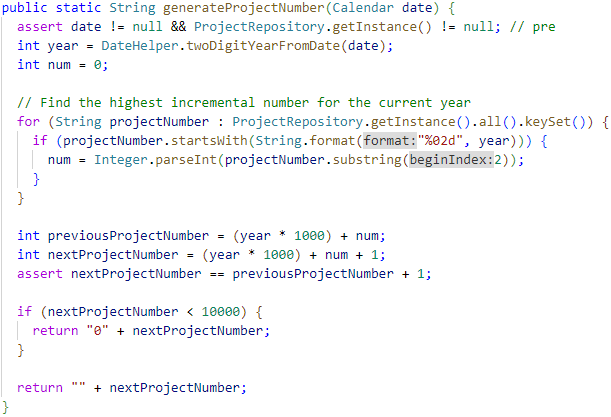
\includegraphics[width = 14cm, keepaspectratio]{ImplementationAndTest/Diagrams/contract_generateProjectNumber.png}
    \label{fig:contract_generateProjectNumber}
\end{figure}

\subsection{createInitials}
pre:
\begin{equation}
    nEmployeesWithName(employee) < maxInitials(employee)
\end{equation}
post:
\begin{equation}
    \{s | \exists e \in employeeRepository : s \in e.getInitials()\}
\end{equation}
Hvor maxInitials(employee) er $n$ vælg 2, hvor $n$ er længden af efternavnet, og duplikater fjernes i generationen af kombinationer.
I "Laudrup" (længde 7, $7 \choose 2$=21) går "lu", "au", "up" igen to gange, hvorfor der fås 18 og ikke de forventede 21. Der forklarer hvorfor white-box testens input er konstrueret som det er.\\[4mm]
Med asserts ser det ud som følger
\begin{figure}[H]
    \centering
    \caption{createInitials med asserts}
    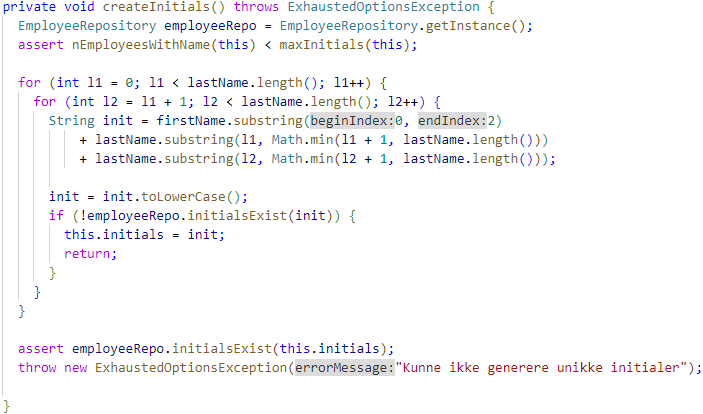
\includegraphics[width = \textwidth, keepaspectratio]{ImplementationAndTest/Diagrams/contract_createInitials.png}
    \label{fig:contract_createInitials}
\end{figure}
\subsection{createProjectActivity}
pre: 
\begin{equation}
    title \neq null \wedge startWeek \neq null \wedge endWeek \neq null \wedge loggedInUser \neq null \wedge activities \neq null
\end{equation}

post: 
\begin{equation}
\begin{gathered}
    activity \in activities \wedge \\
    \neg project@pre.hasProjectActivity(title) \wedge \\
    (hasProjectLeader() \to projectLeader.isSameAs(loggedInUser))
\end{gathered}
\end{equation}

\begin{listing}[H]
    \centering
    \caption{createProjectActivity() kildekode med assertions}\label{lst:create_project_activity_assertions}
    \begin{minted}[breaklines]{java}
  public ProjectActivity createProjectActivity(String title, String startWeek, String endWeek, Employee loggedInUser)
      throws AlreadyExistsException, OperationNotAllowedException, InvalidPropertyException {

    assert title != null;
    assert startWeek != null;
    assert endWeek != null;
    assert loggedInUser != null;
    assert activities != null;

    if (hasProjectLeader()) {
      if (!projectLeader.isSameAs(loggedInUser)) {
        throw new OperationNotAllowedException("Kun projektlederen kan oprette en projekt aktivitet for dette projekt");
      }
    }

    if (hasProjectActivity(title)) {
      throw new AlreadyExistsException("Projekt aktivitet findes allerede");
    }

    ProjectActivity activity = new ProjectActivity(title, startWeek, endWeek);
    this.activities.add(activity);

    /**
     * NOTE: This post condition does not check for 
     * !project@pre.hasProjectActivity(title)
     */
    assert (
      activities.contains(activity) &&
      (!hasProjectLeader() || projectLeader.isSameAs(loggedInUser) )
    );

    return activity;
  }
    \end{minted}
\end{listing}


\subsection{findWorktimeRegistrationById()}
\noindent pre: 
\begin{align}
    allWorktimeRegistrations().size()\; >\; 0 \;\wedge\; id \; \in \; \mathbb{N} \; \wedge \; 0 \; < \; id  \; <=\; allWorktimeRegistrations().size()
\end{align}
post: 
\begin{equation}
    \exists i\; :\; (i\; \in\; result\; \iff\; \exists worktimeRegistration.getId() \; = \; i)
\end{equation}

\begin{listing}[H]
    \centering
    \caption{findWorktimeRegistrationById() kildekode med assertions}\label{lst:find_work_time_registration_by_id_assertions}
    \begin{minted}[breaklines]{java}
public WorktimeRegistration findWorktimeRegistrationById(int id) throws NotFoundException {

    assert allWorktimeRegistrations().size() > 0 && id == (int) id && 0 < id && id <= allWorktimeRegistrations().size(); // Precondition
    
    List<WorktimeRegistration> list = allWorktimeRegistrations();

    for (WorktimeRegistration worktimeRegistration : list) {
        if (worktimeRegistration.getId().equals(id)) {
            assert worktimeRegistration.getId().equals(id); // Postcondition
            
            return worktimeRegistration;
        }
    }

    throw new NotFoundException("Ukendt tidsregistrering");

}
    \end{minted}
\end{listing}


